\chapter{Materiales y Metodología} % Título del capítulo
\label{Chapter4}
\lhead{Capítulo 4. \emph{Materiales y Metodología}}

Este capítulo describe los materiales empleados (base de datos de imágenes y entorno de implementación) y la metodología propuesta: un framework de procesamiento por etapas que, a partir de una radiografía con deficiencias de contraste, produce automáticamente una imagen mejorada seleccionada por métodos de decisión multicriterio.

\section{Materiales}

\subsection{Base de datos de imágenes}

Se utiliza la base de datos pública \textit{Panoramic radiography database} \citep{Fretes2021}, compuesta por 598 ortopantomografías digitales en escala de grises de 2041 $\times$ 1024 píxeles en formato JPEG, adquiridas con un equipo Owandy I-max Touch en el Departamento de Radiología de la Facultad de Odontología de la Universidad Nacional de Asunción y publicada bajo licencia CC-BY-4.0 junto con el trabajo de \citet{MelloRoman2021}. Las imágenes presentan la variabilidad anatómica y de adquisición propia de la práctica clínica, lo que las hace representativas del escenario de aplicación del framework.

\subsection{Entorno de implementación}

El framework se implementó en Python 3, empleando las bibliotecas NumPy y SciPy para el cálculo numérico, OpenCV y scikit-image para el procesamiento de imágenes, y pandas y Matplotlib para el análisis y la visualización de resultados. La implementación completa, junto con los scripts de experimentación y las pruebas unitarias, se encuentra disponible públicamente.
% TODO: citar URL del repositorio en la versión final.

\section{Arquitectura del framework}
\label{sec:arquitectura}

El framework se estructura como un procesamiento por etapas:

\begin{equation*}
\text{entrada} \rightarrow \text{optimización} \rightarrow \text{transformación} \rightarrow \text{decisión} \rightarrow \text{salida}
\end{equation*}

\begin{figure}[H]
    \centering
    % Figura generada con scripts/generate_framework_figure.py a partir de una
    % ejecución real del pipeline (imagen 114 del dataset, SMPSO 30x30, 8 MCDM)
    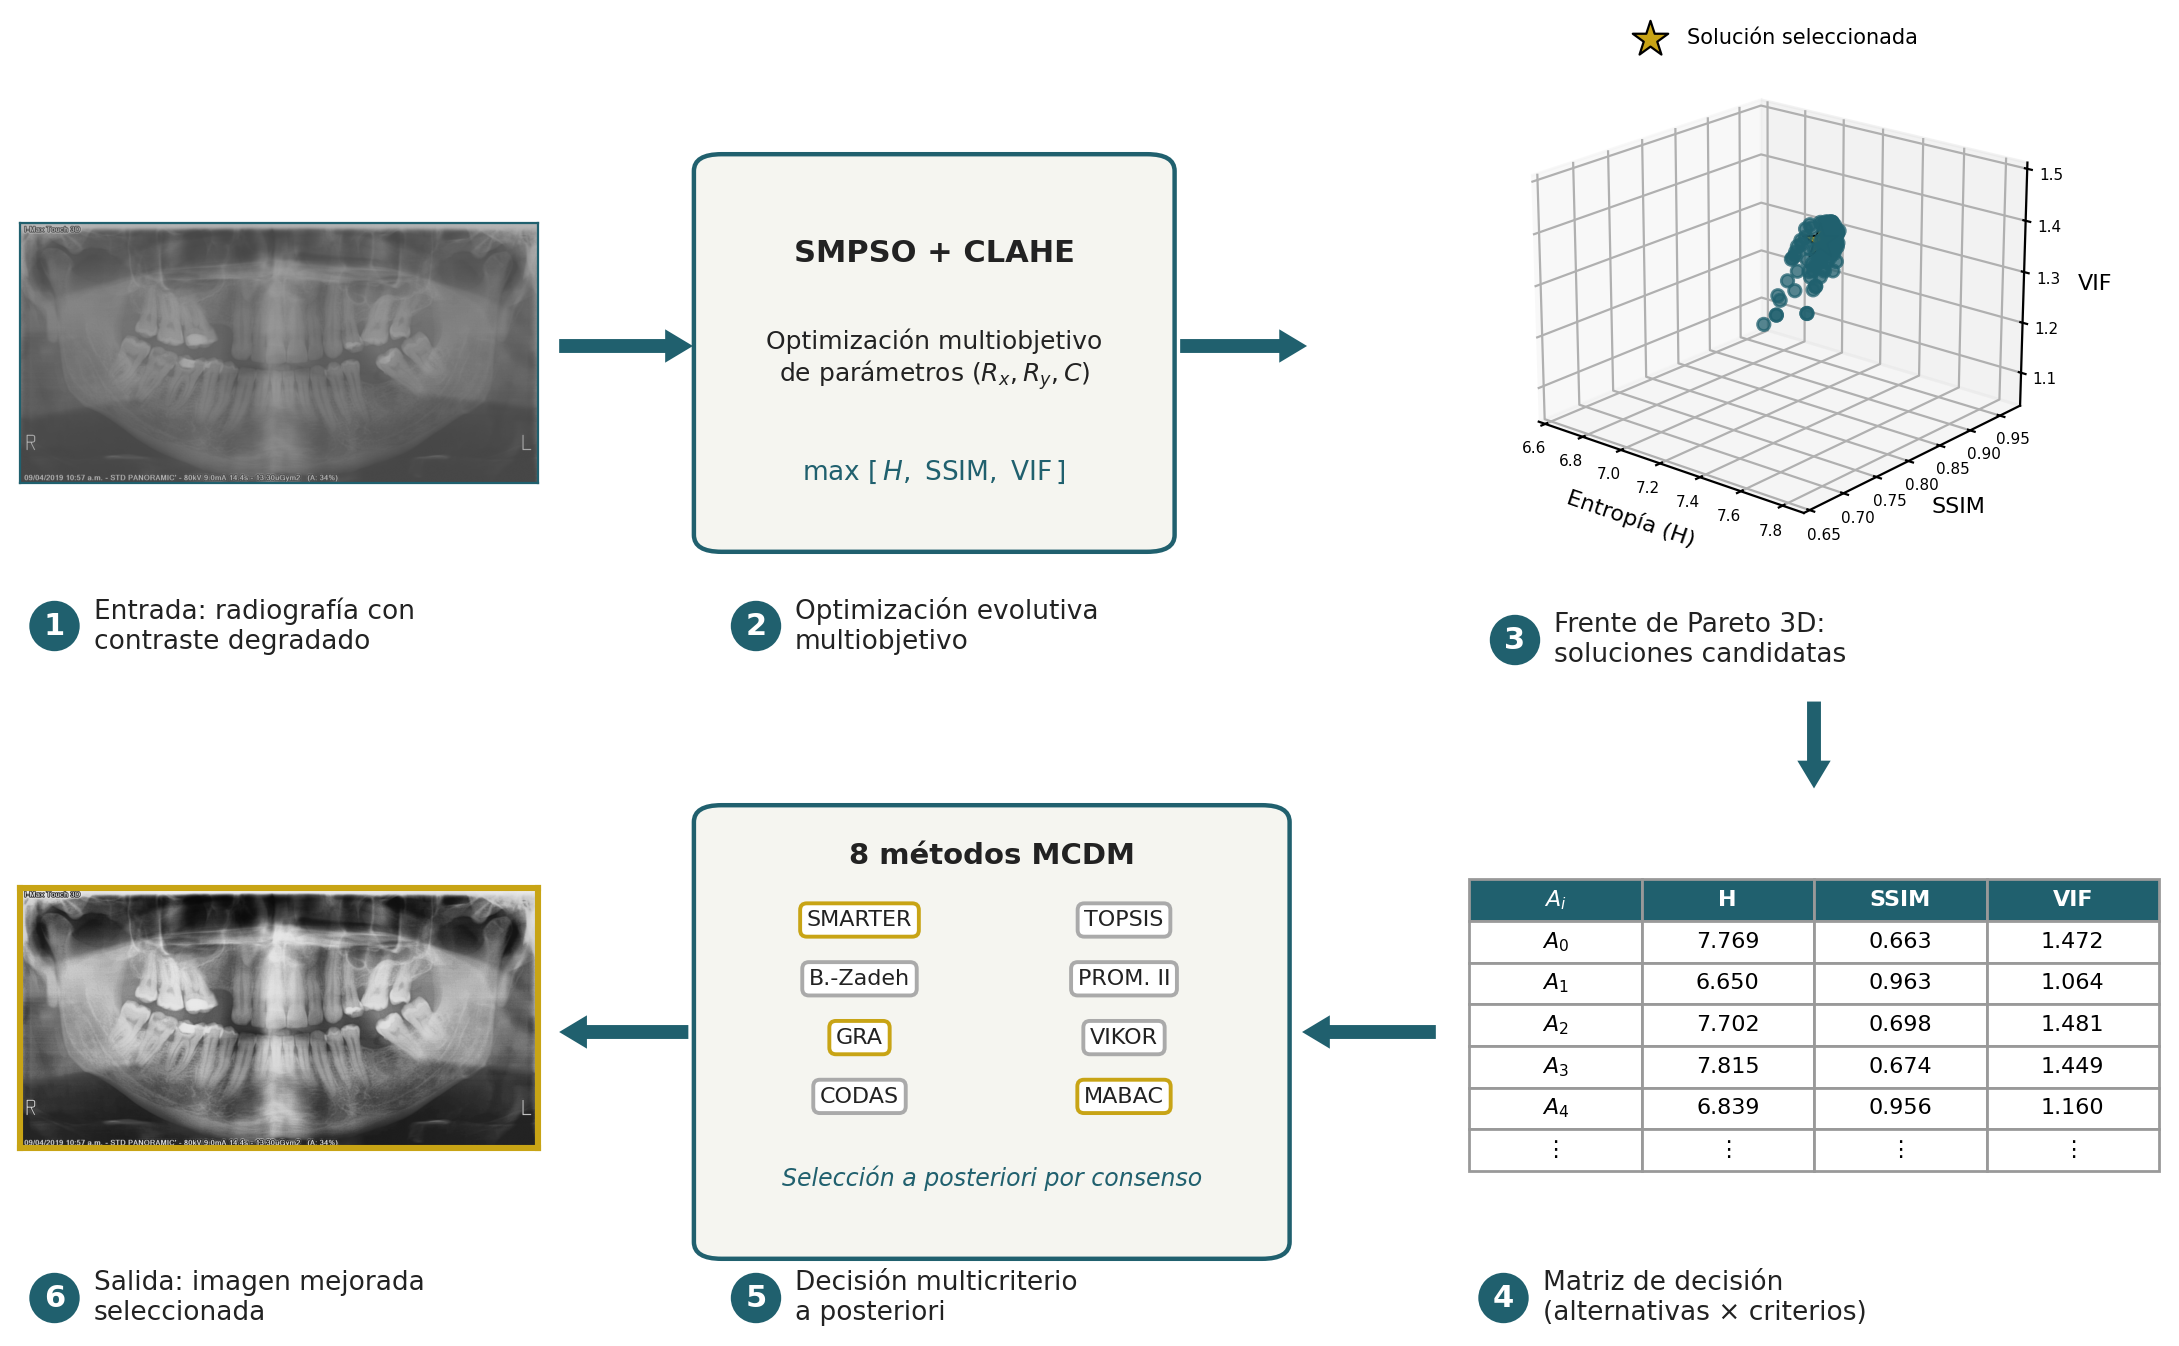
\includegraphics[width=\textwidth]{./Figures/capitulo4/framework}
    \caption[Arquitectura por etapas del framework propuesto]{Arquitectura por etapas del framework propuesto, ilustrada con una ejecución real del pipeline: (1) la ortopantomografía de entrada con contraste degradado; (2) SMPSO optimiza los parámetros $(R_x, R_y, C)$ de CLAHE maximizando entropía, SSIM y VIF; (3) el Frente de Pareto 3D resultante con las soluciones candidatas; (4) el frente se mapea a una matriz de decisión; (5) los ocho métodos MCDM seleccionan a posteriori una alternativa (en dorado, los métodos que votaron por la solución de consenso); (6) la imagen mejorada correspondiente a la solución seleccionada.}
    \label{fig:framework}
\end{figure}

\begin{enumerate}
    \item \textbf{Entrada:} una imagen radiográfica en escala de grises con deficiencias de contraste (supuesto de partida del problema).

    \item \textbf{Optimización:} el algoritmo SMPSO explora el espacio de parámetros de CLAHE $(R_x, R_y, C)$, evaluando cada configuración candidata mediante las tres funciones objetivo. El resultado es una aproximación del Frente de Pareto con hasta 100 soluciones no dominadas.

    \item \textbf{Transformación:} cada solución del Frente de Pareto corresponde a una imagen mejorada, obtenida aplicando CLAHE con los parámetros de la solución sobre la imagen de entrada.

    \item \textbf{Decisión:} el Frente de Pareto se mapea a una matriz de decisión (alternativas $\times$ criterios) sobre la cual se aplican los ocho métodos MCDM. Cada método selecciona una solución final; adicionalmente se calcula la solución de consenso.

    \item \textbf{Salida:} la imagen mejorada correspondiente a la solución seleccionada, junto con sus parámetros y métricas.
\end{enumerate}

Las siguientes secciones detallan cada etapa.

\section{Etapa de optimización}

\subsection{Espacio de búsqueda}

Las variables de decisión son los tres parámetros de CLAHE, con los siguientes límites:

\begin{table}[H]
\centering
\caption{Espacio de búsqueda de los parámetros de CLAHE.}
\label{tab:espacio_busqueda}
\begin{tabular}{llll}
\hline
\textbf{Parámetro} & \textbf{Descripción} & \textbf{Dominio} & \textbf{Tipo} \\
\hline
$R_x$ & Regiones contextuales en el eje horizontal & $[2, 64]$ & Entero \\
$R_y$ & Regiones contextuales en el eje vertical & $[2, 64]$ & Entero \\
$C$ & Límite de recorte (\textit{clip limit}) & $[1.0, 4.0]$ & Real \\
\hline
\end{tabular}
\end{table}

$R_x$ y $R_y$ se manejan como variables reales durante la búsqueda y se redondean al entero más próximo para la evaluación, estrategia estándar para variables discretas en PSO.

\subsection{Funciones objetivo}

Cada configuración candidata $(R_x, R_y, C)$ se evalúa aplicando CLAHE a la imagen de entrada $I$ y calculando sobre la imagen resultante $I'$ las tres métricas descritas en la Sección~\ref{sec:metricas}, todas a maximizar:

\begin{equation}
\vec{f}(R_x, R_y, C) = \left( H(I'), \; \text{SSIM}(I, I'), \; \text{VIF}(I, I') \right)
\label{eq:funciones_objetivo}
\end{equation}

La entropía premia el aumento de información, el SSIM la preservación estructural respecto a la entrada y el VIF la fidelidad de información visual. Para reducir el costo computacional de la búsqueda, durante la optimización las evaluaciones se realizan sobre una versión de la imagen reescalada a un máximo de 512 píxeles en su dimensión mayor; la imagen final de salida se genera aplicando los parámetros seleccionados sobre la imagen a resolución completa.

\subsection{Configuración de SMPSO}

Se emplea la configuración canónica de SMPSO \citep{Nebro2009}, cuya justificación proviene del estudio original del algoritmo:

\begin{table}[H]
\centering
\caption{Parámetros de SMPSO empleados.}
\label{tab:config_smpso}
\begin{tabular}{lll}
\hline
\textbf{Parámetro} & \textbf{Valor} & \textbf{Justificación} \\
\hline
Tamaño del enjambre & 100 & \citep{Nebro2009} \\
Iteraciones & 100 & Presupuesto; validado en la Sección~\ref{sec:convergencia} \\
Tamaño del archivo externo & 100 & \citep{Nebro2009}; ver Sección~\ref{sec:convergencia} \\
$C_1$, $C_2$ & $U(1.5, 2.5)$ & \citep{Nebro2009} \\
Peso de inercia $w$ & 0.1 & \citep{Nebro2009} \\
Coeficiente de constricción & Ec.~\ref{eq:constriccion} & \citep{Clerc2002} \\
Mutación polinomial & 15\% del enjambre, $\eta_m = 20$ & \citep{Nebro2009} \\
Selección de líderes & Torneo binario por crowding distance & \citep{Deb2002} \\
\hline
\end{tabular}
\end{table}

El tamaño del enjambre y del archivo externo (100) corresponden a la configuración del estudio original de SMPSO y a los valores por defecto de jMetal, la implementación de referencia de sus autores \citep{Nebro2009}. El número de iteraciones requiere una aclaración: el estudio original emplea un presupuesto de 25\,000 evaluaciones ($\approx$250 iteraciones), mientras que aquí se utilizan 100 iteraciones (10\,000 evaluaciones por imagen) como compromiso entre calidad de la aproximación y costo computacional, dado que cada evaluación implica aplicar CLAHE y calcular tres métricas sobre la imagen. La suficiencia de este presupuesto se valida empíricamente en la Sección~\ref{sec:convergencia} mediante el análisis de la evolución del hipervolumen.

\section{Etapa de decisión}

\subsection{Matriz de decisión}

El Frente de Pareto resultante de la optimización, con $m$ soluciones y $k = 3$ objetivos, se mapea directamente a la matriz de decisión $X = [x_{ij}]_{m \times 3}$, donde cada alternativa es una solución no dominada y cada criterio una función objetivo. Los tres criterios son de tipo beneficio.

\subsection{Pesos de los criterios}
\label{sec:pesos}

Al no disponer de una elicitación directa de preferencias de profesionales odontólogos, los pesos se derivan del orden de importancia de los criterios mediante las aproximaciones sustitutas de \citet{Roberts2002} descritas en la Sección~\ref{sec:matriz_decision}.

El orden de importancia adoptado es $\text{VIF} \succ H \succ \text{SSIM}$, justificado por el rol que cumple cada métrica respecto al objetivo del framework, esto es, la utilidad diagnóstica de la imagen:

\begin{itemize}
    \item El \textbf{VIF} es la métrica con mayor correlación reportada con el juicio perceptual humano \citep{Sheikh2006} y la única que cuantifica directamente la información visual efectivamente disponible para un observador; se le asigna, por tanto, la mayor importancia.
    \item La \textbf{entropía} mide la cantidad de información presente en la imagen, condición necesaria pero no suficiente para la utilidad diagnóstica: una imagen puede tener entropía alta y ser ruidosa.
    \item El \textbf{SSIM} cumple un rol de salvaguarda estructural más que de objetivo primario: penaliza toda alteración respecto a la entrada, incluso aquella que restituye contraste diagnóstico. Se le asigna la menor importancia para no favorecer soluciones que se limiten a preservar la imagen degradada.
\end{itemize}

Aplicando ROC a este orden con $n = 3$ criterios se obtienen los pesos $(w_{\text{VIF}}, w_{H}, w_{\text{SSIM}}) = (0.611, 0.278, 0.111)$. Dado que la elección del orden de importancia constituye la principal decisión subjetiva del framework, en la Sección~\ref{sec:sensibilidad} se reporta un análisis de sensibilidad que compara este esquema con \textit{Rank Sum}, pesos iguales y una ponderación preliminar alternativa, evaluando la estabilidad de las selecciones resultantes.

El método SMARTER constituye una excepción deliberada: por definición deriva sus propios pesos ROC del orden de importancia \citep{Edwards1994}, de modo que no recibe pesos externos.

\subsection{Métodos de decisión y consenso}

Sobre la matriz de decisión se aplican los ocho métodos MCDM descritos en la Sección~\ref{sec:mcdm}, cada uno con su normalización canónica (Tabla~\ref{tab:normalizaciones}) y el mismo vector de pesos. Cada método produce un ranking completo de las alternativas y una selección final. Adicionalmente se calcula la \textbf{solución de consenso}: la alternativa seleccionada por la mayor cantidad de métodos.

\section{Diseño experimental}
\label{sec:diseno_experimental}

\subsection{Degradación controlada}
\label{sec:degradacion}

Para validar el framework de forma objetiva se requiere una referencia de calidad conocida. Con este fin, cada imagen original $I_o$ de la muestra se somete a una degradación de contraste controlada, produciendo la imagen $I_d$ que actúa como entrada del framework. Esto permite evaluar cuánta calidad recupera la imagen mejorada $I'$ respecto a la original $I_o$, que actúa como \textit{ground truth}.

Se implementaron cinco tipos de degradación representativos de las deficiencias observadas en la práctica:

\begin{itemize}
    \item \textbf{Bajo contraste global:} compresión lineal del rango dinámico.
    \item \textbf{Subexposición:} transformación gamma ($\gamma > 1$) con desplazamiento negativo.
    \item \textbf{Sobreexposición:} transformación gamma ($\gamma < 1$) con saturación de altas luces.
    \item \textbf{Bajo contraste local:} suavizado y reducción de contraste por regiones.
    \item \textbf{Histograma sesgado:} desplazamiento de la distribución hacia tonos oscuros o claros.
\end{itemize}

El tipo de degradación y sus parámetros se asignan aleatoriamente a cada imagen, con una semilla derivada del identificador de la imagen para garantizar reproducibilidad y variabilidad simultáneamente. La Figura~\ref{fig:degradaciones} ilustra el efecto de cada tipo de degradación sobre una misma ortopantomografía, junto con la firma característica que cada una imprime en el histograma de intensidades.

\begin{figure}[H]
    \centering
    % Figura generada con scripts/generate_degradations_figure.py
    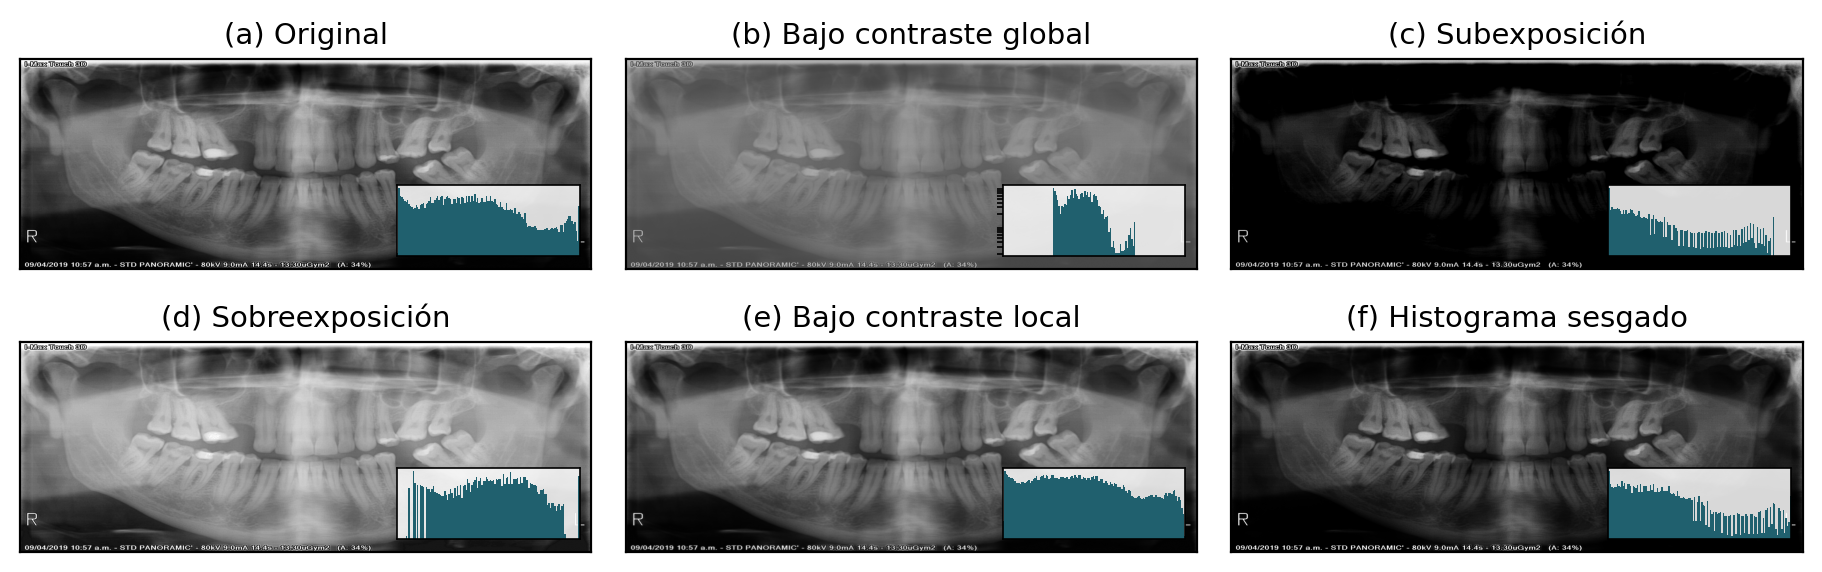
\includegraphics[width=\textwidth]{./Figures/capitulo4/degradaciones}
    \caption[Tipos de degradación controlada de contraste]{Imagen original (a) y los cinco tipos de degradación controlada de contraste aplicados en la experimentación (b--f). Cada panel incluye su histograma de intensidades en escala logarítmica: la compresión del rango dinámico en (b), el desplazamiento hacia tonos oscuros en (c) y (f), la saturación de altas luces en (d) y el aplanamiento local en (e).}
    \label{fig:degradaciones}
\end{figure}

\subsection{Tamaño de la muestra}

De la población de $N = 598$ imágenes se extrae una muestra aleatoria cuyo tamaño se determina mediante la fórmula de Cochran con corrección para poblaciones finitas \citep{Cochran1977}:

\begin{equation}
n = \frac{N \, Z^2 \, p(1-p)}{e^2(N-1) + Z^2 \, p(1-p)}
\label{eq:cochran}
\end{equation}

Con un nivel de confianza del 95\% ($Z = 1.96$), proporción esperada $p = 0.5$ (máxima variabilidad) y margen de error $e = 0.10$, resulta $n = 83$ imágenes.

\subsection{Métricas de evaluación del experimento}

Para cada imagen procesada se registran:

\begin{itemize}
    \item Las métricas objetivo (H, SSIM, VIF) de la solución seleccionada por cada método MCDM y de la solución de compromiso.
    \item Las métricas de \textbf{validación contra la original}: $\text{SSIM}(I_o, I_d)$ vs. $\text{SSIM}(I_o, I')$ y $\text{VIF}(I_o, I_d)$ vs. $\text{VIF}(I_o, I')$, que cuantifican la recuperación de calidad respecto al \textit{ground truth}.
    \item Los parámetros CLAHE seleccionados, el tamaño del Frente de Pareto y el tiempo de procesamiento.
    \item La selección de cada método MCDM, para el análisis de concordancia.
\end{itemize}

\subsection{Análisis de concordancia entre métodos MCDM}

La concordancia entre los ocho métodos se analiza mediante: (i) la matriz de acuerdo por pares, donde cada celda indica el porcentaje de imágenes en que dos métodos seleccionaron la misma alternativa; (ii) la distribución del número de votos de la solución de consenso; y (iii) el análisis por tipo de degradación, para determinar si la concordancia depende del tipo de deficiencia de contraste.

\section{Implementación}

El código se organiza en módulos que reflejan las etapas del framework: \texttt{clahe} (transformación), \texttt{metrics} (funciones objetivo), \texttt{optimization} (SMPSO y Frente de Pareto), \texttt{mcdm} (los ocho métodos de decisión, con una clase base común que define la interfaz de normalización, pesos y ranking) y \texttt{utils} (entrada/salida, degradaciones y visualización). La correctitud de los componentes se verifica mediante una suite de pruebas unitarias e integración (59 pruebas) que cubre las métricas, el procesador CLAHE, los métodos MCDM y el flujo completo de optimización.
